
\lecture{Circuitos lógicos}

\section{\insertlecture}

\frame{\title{\insertlecture}\maketitle}

\begin{frame}{Decodificador}{2 bits}
  \small Recebe um conjunto de entradas que representa um número
  binário e ativa somente uma saída. Para \alert{$k$} entradas é possível
  ativar \alert{$2^k$} saídas.

\bigskip
  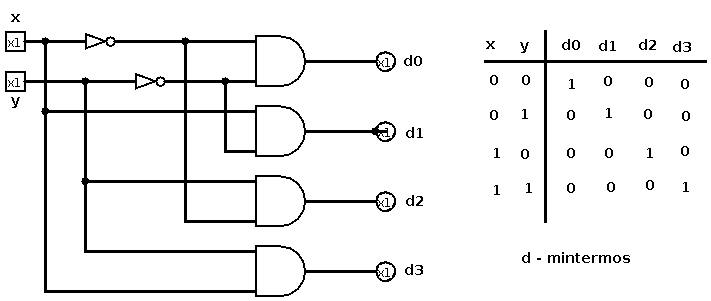
\includegraphics[scale=.4]{\imgdir/decoder-2bit.png}
\end{frame}

\begin{frame}{Decodificador}{3 bits}
  
%%% Local Variables:
%%% mode: latex
%%% TeX-master: t
%%% End:
\begin{tikzpicture}

\def\shift{2cm}

\tikzset{
    every node/.style={font=\scriptsize}, 
    wire/.style={->, >=latex, draw},
    decoder/.style={minimum width=\shift,minimum height=\shift,draw},
    header/.style={minimum width=1.5*\shift,white},
    in header/.style={header, fill=green!65!black},
    out header/.style={header, fill=red!80!black}
}

\node[decoder] (DECODER) at (0,0) {decodificador};
\node (out tip) at (\shift, 0) {};
\node (in tip) at (-\shift, 0) {};

\newcounter{lout}\setcounter{lout}{0}
\foreach \i in {-4,-3,-2,-1,0,1,2,3} {
    \path[wire] (.5*\shift,.225*\i+.1) -- (\shift,.225*\i+.1) node[right]{\tiny \arabic{lout}};
    \addtocounter{lout}{1}
}

\path[wire] (in tip) node[above right] {\tiny 3} -- (DECODER);
\path[draw] (in tip.south east)+(.2*\shift,0) -- +(.08*\shift,.2*\shift);

\matrix [right of=DECODER, xshift=2.5*\shift] (truth table) {
    \node[in header]{Entradas};&\node[out header]{Sa\'idas};\\     
    \node[in header]{2\ \ 1\ \ 0};&\node[out header]{7\ \ 6\ \ 5\ \ 4\ \ 3\ \ 2\ \ 1\ \ 0};\\     
    \node{0\ \ 0\ \ 0}; & \node{0\ \ 0\ \ 0\ \ 0\ \ 0\ \ 0\ \ 0\ \ 1};\\
    \node{0\ \ 0\ \ 1}; & \node{0\ \ 0\ \ 0\ \ 0\ \ 0\ \ 0\ \ 1\ \ 0};\\
    \node{0\ \ 1\ \ 0}; & \node{0\ \ 0\ \ 0\ \ 0\ \ 0\ \ 1\ \ 0\ \ 0};\\
    \node{0\ \ 1\ \ 1}; & \node{0\ \ 0\ \ 0\ \ 0\ \ 1\ \ 0\ \ 0\ \ 0};\\
    \node{1\ \ 0\ \ 0}; & \node{0\ \ 0\ \ 0\ \ 1\ \ 0\ \ 0\ \ 0\ \ 0};\\
    \node{1\ \ 0\ \ 1}; & \node{0\ \ 0\ \ 1\ \ 0\ \ 0\ \ 0\ \ 0\ \ 0};\\
    \node{1\ \ 1\ \ 0}; & \node{0\ \ 1\ \ 0\ \ 0\ \ 0\ \ 0\ \ 0\ \ 0};\\
    \node{1\ \ 1\ \ 1}; & \node{1\ \ 0\ \ 0\ \ 0\ \ 0\ \ 0\ \ 0\ \ 0};\\
};

\node [above of=truth table, yshift=\shift] {Tabela-Verdade};
\end{tikzpicture}


\end{frame}

\begin{frame}{Multiplexador}{mux}

Para \alert{$2^k$} entradas, o \alert{multiplexador} seleciona entre \alert{$k$} saídas.

\begin{center}
\begin{tikzpicture}
  
\def\shift{1cm}
\begin{scope}
  \tikzset{every node/.style={font=\scriptsize},
   every path/.style={->,>=latex, draw},
    mux/.style={rotate=90, minimum height=.5*\shift,minimum width=2*\shift, rounded
      corners=2mm, draw},
    l/.style={gray}
}

    \node[mux] (MUX) at (0,0) {};
    \node[l] (M) at ([yshift=.25*\shift]MUX) {m};
    \node[l] (u) [below of=M,yshift=.75\shift] {u};
    \node[l] (x) [below of=u,yshift=.75\shift] {x};

    \node at ([xshift=-1.5*\shift]MUX.20) (A) {x};
  
    \path  (A) -- (MUX.20) node[right,xshift=1] {$0$};

    \node (B) at ([xshift=-1.5*\shift]MUX.160) {y};
  
    \path (B) -- (MUX.160) node[right,xshift=1] {$1$};

    \node (C) at ([xshift=1.5*\shift]MUX.south) {f};
  
    \path  (MUX.south) -> (C);
  
    \node (S) at ([yshift=-1.5*\shift]MUX.west) {seleção $s$};
  
    \path[->,>=latex]  (S) -> (MUX.west);

    

   \matrix (select table) [matrix of nodes, above of=MUX,xshift=-.5\shift,yshift=\shift]
   {
     \bf s & \bf f \\
     0 & =x \\
     1 & =y \\
   };

\end{scope}

\begin{scope}

  %GATES
  \draw
  (5,1) node[and gate US,draw] (andA){}
  (5,-1) node[and gate US,draw] (andB){}
  (7,0) node[or gate US,draw] (orC){}
  (andA.output) -| (orC.input 1)
  (andB.output) -| (orC.input 2);
  \node[above] (LC) at (orC.output) {$f$};

  %+WIRE
  \path[draw] (andA.input 1) node[] (anchor A) {} -- +(-.5,0) node[above] {x};
  \path[draw] (andB.input 2) node[] (anchor B) {} -- +(-.5,0) node[above] {y};

  \node[] at (andA.input 2) (wire inAtwo)  {};
  \node[ocirc] [right of=wire inAtwo,xshift=-.8*\shift] {};

  % SIGNAL
  \node[right] (S) [below of=anchor B] {seleção $s$};
  \path[draw] (S) -- (andB.input 1) node[circ] {} -- (andA.input 2);

   \node[green!30!black] (EXP) [below of=orC,xshift=.125*\shift,yshift=-\shift] {$f~(s,x,y) = x\overline{s} + ys$};
   

  \end{scope}
  
\end{tikzpicture}

\end{center}

\end{frame}
 
